%%%%%%%%%%%%%%%%%%%%%%%%%%%%%%%%%%%%%%%%%
% Short Sectioned Assignment
% LaTeX Template
% Version 1.0 (5/5/12)
%
% This template has been downloaded from:
% http://www.LaTeXTemplates.com
%
% Original author:
% Frits Wenneker (http://www.howtotex.com)
%
% License:
% CC BY-NC-SA 3.0 (http://creativecommons.org/licenses/by-nc-sa/3.0/)
%
%%%%%%%%%%%%%%%%%%%%%%%%%%%%%%%%%%%%%%%%%

%----------------------------------------------------------------------------------------
%   PACKAGES AND OTHER DOCUMENT CONFIGURATIONS
%----------------------------------------------------------------------------------------

\documentclass[paper=letter, fontsize=11pt]{scrartcl} % A4 paper and 11pt font size
\synctex=1
\usepackage[T1]{fontenc} % Use 8-bit encoding that has 256 glyphs
\usepackage{fourier} % Use the Adobe Utopia font for the document - comment this line to return to the LaTeX default
\usepackage[english]{babel} % English language/hyphenation
\usepackage{amsmath,amsfonts,amsthm} % Math packages
%\usepackage[nolists, nomarkers]{endfloat}
\usepackage{hyperref}
\usepackage{bm}
\usepackage{graphicx}
\usepackage[section]{placeins}
\usepackage{sectsty} % Allows customizing section commands
\allsectionsfont{\normalfont\scshape} % Make all sections centered, the default font and small caps

\usepackage{fancyhdr} % Custom headers and footers
\pagestyle{fancyplain} % Makes all pages in the document conform to the custom headers and footers
\fancyhead{} % No page header - if you want one, create it in the same way as the footers below
\fancyfoot[L]{} % Empty left footer
\fancyfoot[C]{} % Empty center footer
\fancyfoot[R]{\thepage} % Page numbering for right footer
\renewcommand{\headrulewidth}{0pt} % Remove header underlines
\renewcommand{\footrulewidth}{0pt} % Remove footer underlines
\setlength{\headheight}{13.6pt} % Customize the height of the header

\numberwithin{equation}{section} % Number equations within sections (i.e. 1.1, 1.2, 2.1, 2.2 instead of 1, 2, 3, 4)
\numberwithin{figure}{section} % Number figures within sections (i.e. 1.1, 1.2, 2.1, 2.2 instead of 1, 2, 3, 4)
\numberwithin{table}{section} % Number tables within sections (i.e. 1.1, 1.2, 2.1, 2.2 instead of 1, 2, 3, 4)

\setlength\parindent{0pt} % Removes all indentation from paragraphs -
                          % comment this line for an assignment with
                          % lots of text
\setlength\parskip{12pt}

%----------------------------------------------------------------------------------------
%   TITLE SECTION
%   ----------------------------------------------------------------------------------------
%----------------------------------------------------------------------------------------
%   TITLE SECTION
%----------------------------------------------------------------------------------------

\newcommand{\horrule}[1]{\rule{\linewidth}{#1}} % Create horizontal rule command with 1 argument of height

\title{ 
\normalfont \normalsize 
\textsc{Exoplanet Patchy Cloud Project} \\ [25pt] % Your university, school and/or department name(s)
\horrule{0.5pt} \\[0.4cm] % Thin top horizontal rule
\huge Systematic Error Correction\\ % The assignment title
\horrule{2pt} \\[0.5cm] % Thick bottom horizontal rule
}

\author{Yifan Zhou} % Your name

\date{\normalsize\today} % Today's date or a custom date

\begin{document}

\maketitle % Print the title
\section{Summary}

According to previous results, there are two kinds of systematic errors
that downgrade the quality of photometry and need to be corrected.
\begin{enumerate}
\item images that are taken with different dithering positions have
  significant difference in photometry. The most possible cause is 
  bad flat fielding.
\item Short timescale variation on the light curves. Red noise needs
  to be caught and corrected. Following effects can contribute to red
  noise:
  ramp effect, jitter of the telescope, telescope temperature
  fluctuation, intra-pixel  response fluctuation, cosmic rays.
\end{enumerate}

  \section{Red Noises}
  \subsection{Ramp Effect and Pointing Problem}
  According to Deming et al. 2013, Wilkins 2014, ramp effect becomes significant
  when exposure level is larger than 30000 e$^{-}$ per pixel. For both
  F125W and F160W images, the largest count rate per pixel at the
  planetary companions place is 2000 - 2200 e$^{-}$s$^{-}$. For F125W
  images, the exposure time is 30s for each image while for F160W is
  15s. Therefore, the pixel that is the peak of the PSF of the
  companion object in the F125W image may be affected by ramp effect.

  In Figure \ref{fig:peak}, I plotted the count for one pixel that has
  the largest flux at the PSF region of ABPIC-B for every image. In short time-scale
  (i.e. in one exposure set, does not demonstrate in the plot), peak
  fluxes do not have a clear and common ramp effect pattern. For first
  3 orbits, the counts have large scatterings for different dithering
  positions. because the peaks of the PSF could locate at the center
  or edge of the pixel. For the last 3 orbits for which dithering is not
  applied, the peak pixel count demonstrates clear trend.  In the 4th
  and 6th orbits, the peak pixel count decreases with time while for
  5th orbits, it slightly increases with time.

    \begin{figure}[th]
    \centering
    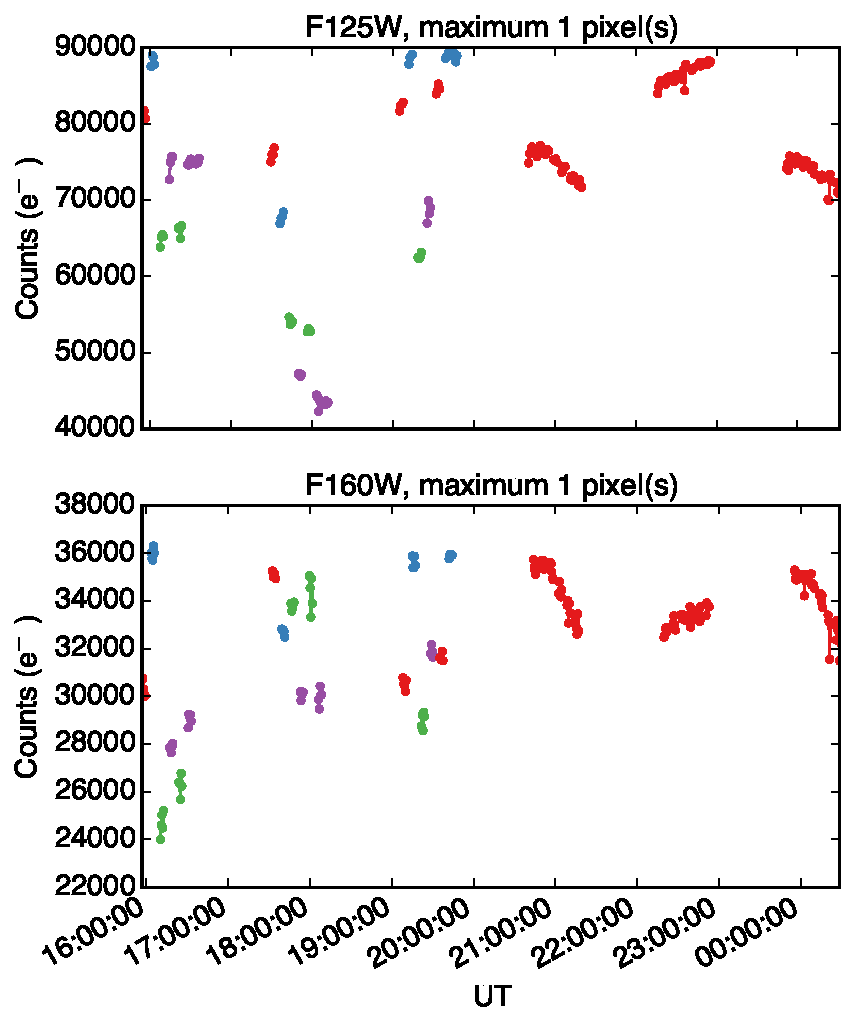
\includegraphics[width=\textwidth]{ramp1Pix}
    \caption{Count for peak pixel on the image of ABPIC-B. Different
      color indicate different dithering position. Count rates are measured
      from the original \texttt{ima} files (no primary subtraction applied)}
    \label{fig:peak}
  \end{figure}

  First of all, I cannot be certain whether ramp effect plays a
  significant role in this trend. The exposure levels of peak pixel for
  F125W images are more than 70000 e$^{-}$, for 5th orbit they are
  near 90000 e$^{-}$, which are almost reach the fully saturation
  level of 100000 e$^{-}$. However, short timescale variations are
  random and no 'hook shaped' (Wilkins et al. 2014) light curves
  appeared.

  This trends for peak pixel count are correlated with the positions of
  PSF centroids. I plot the PSF centroids that are measured by Gaussian
  fitting for 4th, 5th and 6th orbits in Figure \ref{fig:center}. The
  PSF centroids shifted in a specific direction within one orbit. In
  4th and 6th orbits, the centroids shift to +y direction and in 5th
  orbit they shift to (+x, +y) direction. In 4th and 6th orbits, the
  centroids shift to the edge of the pixel while in 5th orbit, they
  slightly shift to the pixel center.

  \begin{figure}[th]
    \centering
    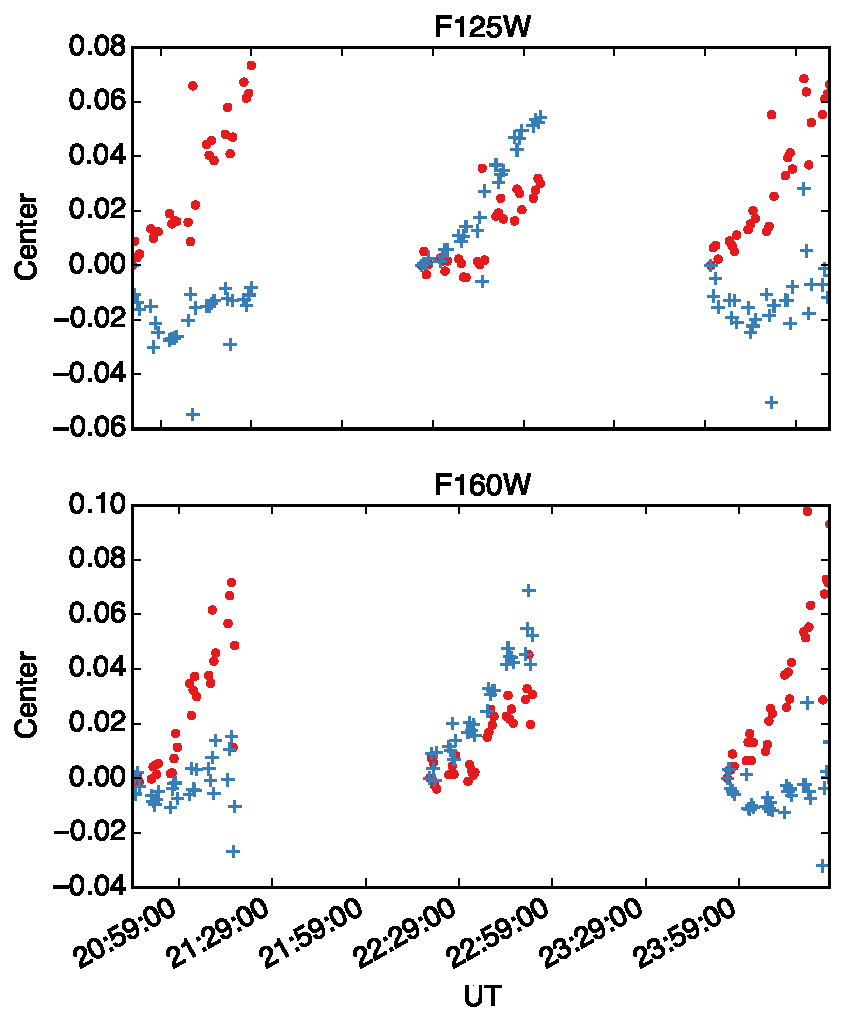
\includegraphics[width=1.0\textwidth]{Ymove}
    \caption{PSF centroid shift for ABPIC-B in 4th, 5th, and 6th
      orbits. Y-axes are the centroid coordinates $(x, y)$ minus the
      those for the first image in each orbit $(x_0, y_0)$. Red dots
      are for x-direction and blue + are for y-direction.}
    \label{fig:center}
  \end{figure}

  To sum,
  \begin{enumerate}
  \item Peak pixels have high exposure levels, especially for F125W,
    ramp effect needs to be considered.
  \item Telescope has a pointing shift within each orbit, and caused
    the peak pixel count varies in a specific trend. Since peak pixel
    contains $\sim 25\%$ of the total flux, if there were a
    considerable intra-pixel response variation, this pointing shift
    could be an error source.
  \end{enumerate}



  \subsection{Cosmic Rays in Up-the-Ramp Fitting}
  \begin{itemize}
  \item In majority of \texttt{ima} files, there are several pixels in
    companion image region that are flagged with 8192 (CR detected by
    up-the-ramp fitting)
    \item it is not clear yet number of pixels that have CR flag is
      correlated with flux scattering
    \item considering use the same PSF images for PSF subtraction.
    \end{itemize}

    \subsection{Jitter}
    \begin{itemize}
    \item 4 exposures have extremely large jitter value
     \item RMS jitter values are about 0.001 arcsec (0.1 pixel)in both
       axes
     \item jitter values seem not to correlate with flux scattering
    \end{itemize}
\end{document}
%%% Local Variables:
%%% mode: latex
%%% TeX-master: t
%%% End:
